\documentclass{article}
\usepackage{listings}
\usepackage{graphics}
\usepackage{graphicx}
\usepackage{hyperref}
\usepackage{amssymb}
\usepackage{float}
\usepackage{amsmath}
\usepackage{longtable}
\usepackage{xcolor}

\definecolor{codegreen}{rgb}{0,0.6,0}
\definecolor{codegray}{rgb}{0.5,0.5,0.5}
\definecolor{codepurple}{rgb}{0.58,0,0.82}
\definecolor{backcolour}{rgb}{0.95,0.95,0.92}

\lstdefinestyle{mystyle}{
    backgroundcolor=\color{backcolour},   
    commentstyle=\color{codegreen},
    keywordstyle=\color{magenta},
    numberstyle=\tiny\color{codegray},
    stringstyle=\color{codepurple},
    basicstyle=\ttfamily\footnotesize,
    breakatwhitespace=false,         
    breaklines=true,                 
    captionpos=b,                    
    keepspaces=true,                 
    numbers=left,                    
    numbersep=5pt,                  
    showspaces=false,                
    showstringspaces=false,
    showtabs=false,                  
    tabsize=2
}

\lstset{style=mystyle}


\title{Chapter 1 \\
Mengenal Artificial Intelligence (AI) dan
Scikit-Learn}
\author{Aditya Luthfi Maulana Harahap (1184090)}
\date{March 2021}

\begin{document}

\maketitle 
\section{Teori}
Artificial Intelligence (AI) atau Kecerdasan Buatan ialah teknologi yang dibuat oleh manusia yang dimodelkan dalam bentuk mesin dan diprogram agar bisa berpikir seperti halnya manusia, yang bisa melakukan pekerjaan-pekerjaan yang umumnya memerlukan tenaga manusia atau kecerdasan manusia. 

Sama seperti manusia, Kecerdasan Buatan atau AI juga membutuhkan pengalaman dan data untuk dijadikan pengetahuan agar pengetahuannya bisa lebih baik lagi. Proses belajarnya berjalan dengan sendirinya berdasarkan pengalamannya saat digunakan oleh manusia. kunci penting dalam proses AI yaitu learning, reasoning, and self correcting.

\subsection{Sejarah}
Sejarah kecerdasan buatan dimulai pada zaman kuno namun sebagai mitos, cerita dan desas-desus tentang makshluk buatan yang diberkahi oleh pengrajin. Karya ini memuncak saat penemuan komputer digital yang diprogram pada tahun 1940-an.
Istilah kecerdasan buatan pertama kali dikemukakan pada tahun 1956 di Konferensi Darthmouth. Sejak saat itulah ia terus dikembangkan sampai saat ini.

"Intelligence" berasal dari bahasa Latin yaitu "intelligo" yang berarti "saya paham". Arti dasar dari intelligence ialah kemampuan untuk memahami dan melakukan aksi.

Pada akhir 1955, Newell dan Simon mengembangkan  The Logic Theorist, program AI pertama. Program ini berdampak besar dan menjadi batu loncatan penting dalam mengembangkan bidang AI. Pada tahun 1956 John McCarthy dari  Massacuhetts Institute of Technology dianggap sebagai bapak AI, menyelenggarakan konferensi untuk menarik para ahli komputer bertemu, dengan  nama kegiatan “The Dartmouth summer research project on artificial intelligence.”   Konferensi Dartmouth itu mempertemukan para pendiri dalam AI, dan bertugas untuk meletakkan dasar bagi masa depan  pemgembangan dan penelitian AI. Pada  tahun 1960 hingga 1970, muncul berbagai dikusi bagaimana komputer dapat meniru sedetail mungkin pada kemampuan otak manusia, dimana saat itu dapat dikategorikan sebagai “classical AI”. Pada tahun 1980, computer semakin mudah diperoleh dengan harga yang lebih murah, lalu menjadikan berbagai riset di bidang kecerdasan buatan semakin berkembang pesat pada berbagai universitas.

\subsection{Perkembangan Kecerdasan Buatan}
\begin{itemize}
\item{Awal Perkembangan AI ( 1952 - 1969 )}
Diawali dengan kesuksesan Newell dan Simon dengan sebuah program yaitu General Problem Solver yang dirancang untuk memuai penyelesaian masalah secara manusiawi, kecerdasan buatan mengalami banyak kesuksesan.

1959 Nathaniel Rochester dari IBM dan mahasiswa-mahasiswanya juga mengeluarkan program kecerdasan buatan dengan nama Geometry Theorm Prover yang dapat mengeluarkan suatu teorema menggunakan aksioma-aksioma yang ada.

1963 James Slagel juga membuat program yang mampu menyelesaikan masalah integral tertutup untuk matakuliah kalkulus.

Selanjutnya pada 1986 Tom Evan juga membuat program analogi yang dapat menyelesaikan masalah analogi geometris yang ada pada tes IQ.

\item{Perkembangan kecerdasan buatan Melambat ( 1966 - 1974 )}
Pada Tahun 1966 hingga 1974 perkembangan kecerdasan buatan mulai melambat, hal ini disebabkan oleh 3 kesulitan utama yaitu:

Pertama, program-program yang bermunculan hanya mengandung sedikit pengetahuan pada subjeknya. Program tersebut berhasil hanya karena manipulasi sederhananya saja.

Kedua, banyaknya masalah yang harus diselesaikan oleh kecerdasan buatan tersebut.

Ketika, Terdapat beberapa batasan pada struktur dasar yang digukanakan untuk menghasilkan perilaku intelligensia.

\item{Sistem Berbasis Pengetahuan ( 1969 - 1979 )}
Pada tahun 1969-1979 Ed Feingenbaum, Bruce Buchanan dan Joshua Lederberg membuat program untuk memecahkan masalah struktur molekul dari informasi yang didapatkan dari spectrometer massa yang mereka namakan Dendral Programs yang berfokus pada pengetahuan kimia. 

\item{Kecerdasan buatan menjadi sebuah industri ( 1980 - 1988 )}
Industrialisasi kecerdasan buatan diawali dengan ditemukannya sistem pakar yang dinamakan R1 yang mampu mengkonfigurasi sistem-sistem komputer baru dan mulai dioperasikan di DEC, McDermott pada 1982.

\item{Kembalinya Jaringan Syaraf Tiruan ( 1986 - Sekarang )}
Meskipun bidang ilmu komputer menolak jaringan syaraf tiruan, namun para ilmuwan masih mempelajari bidang ilmu tersebut dari sudut pandang lain seperti menggunakan teknik-teknik mekanika statistika untuk menganalisa sifat-sifat penyimpanan dan optimasi pada jaringan syaraf.
Pada tahun 1985-an  empat kelompok riset menemukan kembali algoritma belajar propagasi balik (Back-Propagation Learning). Algoritma ini berhasil diimplementasikan ke dalam bidang ilmu komputer dan psikologi.
\end{itemize}


\subsection{Definisi Supervised dan Unsupervised Learning}
Supervised Learning ialah suatu pendekatan  dimana terdapat data dan variabel yang telah ditargetkan sehingga pendekatan tersebut dapat mengelompokkan sebuah data ke data yang sudah ada. Berbeda dengan Unsupervised Learning yang tidak mempunyai data, sehingga data yang ada harus dikelompokkan menjagi beberapa bagian.

\subsection{Definisi Klasifikasi dan Regresi}
Menurut KBBi, klasifikasi merupakan penyusunan sistem di dalam kelompok atau golongan berdasarkan kaidah atau standar yang telah ditetapkan. 
Regresi adalah sebuah metode analisis statistic yang akan digunakan untuk melihat pengaruh variabel

\subsection{Definisi Dataset, Training Set dan Testing Set}
Dataset ialah suatu objek yang akan mempresentasikan sebuah data dan relasinya di memory atau penyimpnan. Struktur pada dataset ini serupa dengan data yang ada di dalam database. 

Training set adalah bagian dari dataset yang berperan dalam membuat prediksi atau algoritma sesuai dengan tujuan masing-masing.

Testing set adalah bagian dari dataset yang akan di tes guna melihat keakuratan atau ketepatan datanya.

\section{Praktek}
\subsection{Instalasi library scikit dari anaconda}
Proses instalasi library melalui anaconda prompt dengan mengetikkan kode : 
\item pip install -U scikit-learn
\item berikut dokumentasi nya :

\begin{center}
    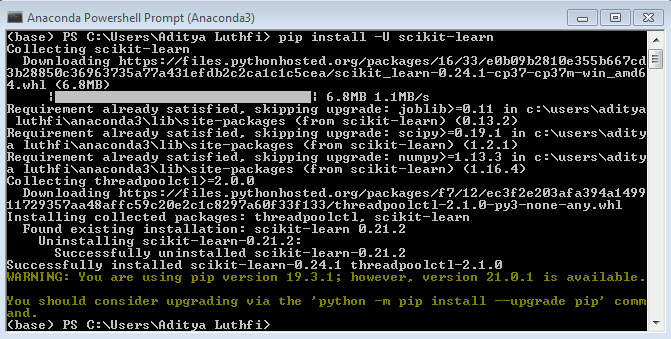
\includegraphics[width=.8\textwidth]{figures/1184090/chapter1/1.PNG}
\end{center}

    

\subsection{Loading an example dataset}
codingan

\begin{center}
    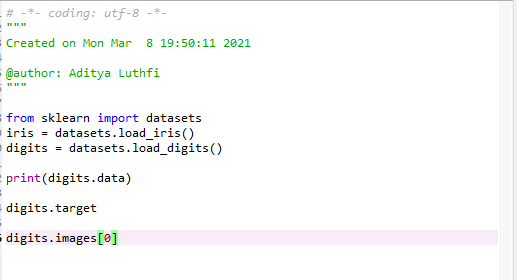
\includegraphics[width=.8\textwidth]{figures/1184090/chapter1/2.PNG}
\end{center}


\begin{enumerate}
\textbf{Penjelasan koding} :
		
		
		\begin{verbatim} from sklearn import datasets \end{verbatim} script diatas maksudnya import class dataset dari scikit learn library
		
		\begin{verbatim} iris = datasets.load_iris() \end{verbatim} script diatas menunjukkan dataset iris dimuat dan dimasukkan  ke variable bernama iris
		
		\begin{verbatim} digits = datasets.load_digits() \end{verbatim} script diatas menunjukkan  dataset digits dimuat dan dimasukkan ke variable digits
		
		\begin{verbatim} print(digits.data) \end{verbatim} memberi akses ke fitur yg dipakai untuk mengklasifikasi sampel digits 
		
		\begin{verbatim} digits.target  \end{verbatim} merupakan info data label
		
		\begin{verbatim} digits.images[0]  \end{verbatim} Merupakan data yang berupa array 2D, shape(n.samples. n.features), walaupun data aslinya bisa berbeda bentuk.
\end{enumerate}
Hasilnya:
\begin{center}
    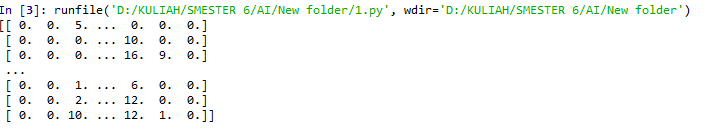
\includegraphics[width=.8\textwidth]{figures/1184090/chapter1/3.PNG}
\end{center}

\subsection{Learning and predicting}

codingan

\begin{center}
    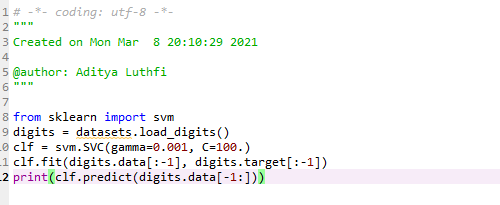
\includegraphics[width=.8\textwidth]{figures/1184090/chapter1/4.PNG}
\end{center}

keterangan
\begin{verbatim} from sklearn import svm \end{verbatim} script diatas maksudnya import class class svm dari package sklearn.
		
		\begin{verbatim} digits = datasets.load_digits() \end{verbatim} script diatas menunjukkan  dataset digits dimuat dan dimasukkan ke variable digits
			
		\begin{verbatim} clf = svm.SVC(gamma=0.001, C=100.)  \end{verbatim} clf sebagai estimator/parameter. svm. kemudian SVC sebagai class nya dan gamma sebagai parameter untuk penetapan nilai yang dilakukan secara manual

		
		\begin{verbatim} clf.fit(digits.data[:-1], digits.target[:-1])  \end{verbatim} clf sebagai estimator/parameter. fit sebagai metode nya kemudian digits.data sebagai item dan [:1] sebagai syntax python yang menampilkan output.
		
		\begin{verbatim} print(clf.predict(digits.data[-1:]))  \end{verbatim} clf sebagai estimator/parameter. predict sebagai metode lain. digits.data sebagai item dan menampilkan output.

Hasilnya:
\begin{center}
    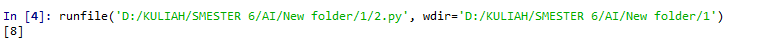
\includegraphics[width=.8\textwidth]{figures/1184090/chapter1/5.PNG}
\end{center}


\subsection{Model persistence}
codingan
\begin{center}
    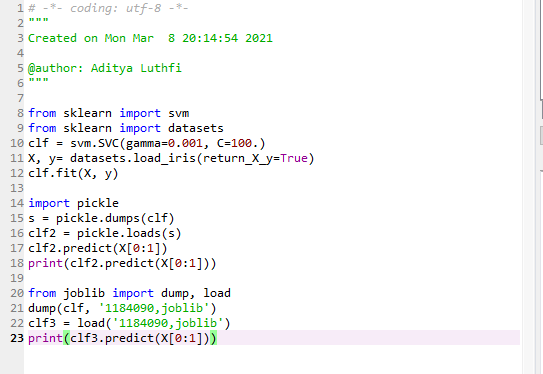
\includegraphics[width=.8\textwidth]{figures/1184090/chapter1/6.PNG}
\end{center}

keterangan
\begin{verbatim}from sklearn import svm\end{verbatim}import svm dari scikit learn library
		
		\begin{verbatim}from sklearn import datasets\end{verbatim}import dataset dari scikit learn library
        
        \begin{verbatim}clf = svm.SVC(gamma=0.001, C=100.)\end{verbatim} memanggil class SVC dan manset argument sonstructor SVC serta ditampung di variable clf
        
        \begin{verbatim}X, y= datasets.load_iris(return_X_y=True) \end{verbatim}meload dataset iris dan datasets dan ditampung di variable x untuk data dan y untuk target

        \begin{verbatim}clf.fit(X, y)\end{verbatim}memanggil methode fit untuk melakukan training data dengan argumen data dan target dari datasets iris

        \begin{verbatim} import pickle\end{verbatim} mengimport pickle
        
        \begin{verbatim} s = pickle.dumps(clf) \end{verbatim} memanggil method dumps dengan argumen clf dan ditampung di variable s
        
        \begin{verbatim} clf2 = pickle.loads(s)\end{verbatim} memanggil metnode loads dengan argumen s dan ditampung di variable clf2
        
        \begin{verbatim} print(clf2.predict(X[0:1]))\end{verbatim}menampilkan hasil dari method predict dengan argumen data variable

        \begin{verbatim}from joblib import dump, load\end{verbatim} mengimport dump dan load dari library joblib dump(clf, '1184095.joblib') ini untuk memanggil methode dumps dengan argumen clf dan nama file joblibnya
        
        \begin{verbatim} clf3 = load('1184095.joblib') \end{verbatim} memanggil methode loads dengan argumen nama file joblibnya dan ditampung di variable clf3
        
        \begin{verbatim}print(clf3.predict(X[0:1]))\end{verbatim}menampilkan hasil dari methode predict dengan argumen data variable x pertama
        
Hasilnya :
\begin{center}
    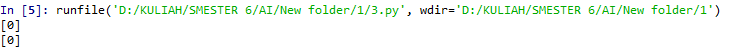
\includegraphics[width=.8\textwidth]{figures/1184090/chapter1/7.PNG}
\end{center}



\subsection{Conventions}
codingan

\begin{center}
    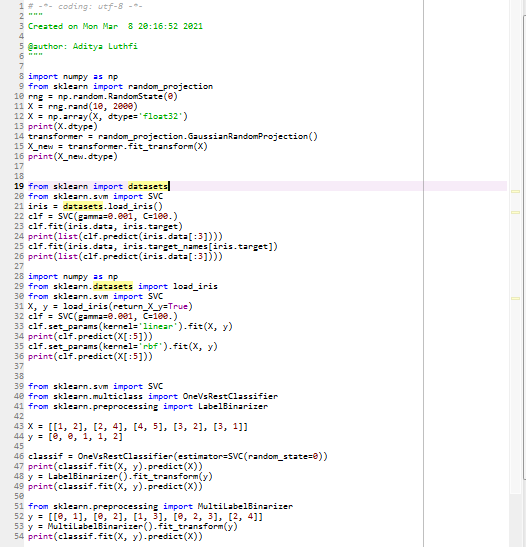
\includegraphics[width=.8\textwidth]{figures/1184090/chapter1/8.PNG}
\end{center}

Hasilnya:
\begin{center}
    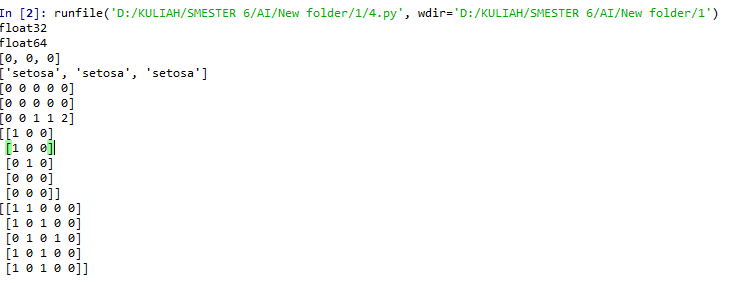
\includegraphics[width=.8\textwidth]{figures/1184090/chapter1/9.PNG}
\end{center}





\section{Error}
Pada saat praktikum, saya mengalami beberapa error, seperti:
\begin{center}
    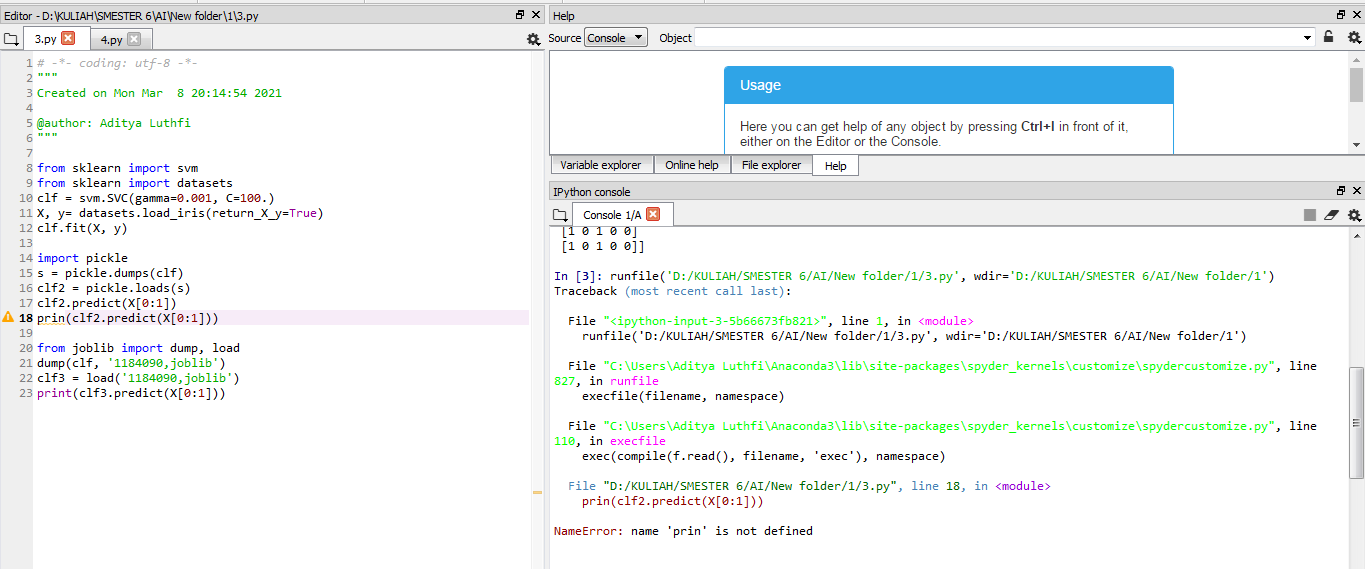
\includegraphics[width=.8\textwidth]{figures/1184090/chapter1/10.PNG}
\end{center}
gagal menampilkan hasil karena salah dari penulisan

\end{document}
